%
\section{Troubleshooting}\label{sec:troubleshooting}
%
\subsection{Mer build engine for cross compilation}\label{subset:ts:mersdk}
%
\subsubsection{Management Webpage}
%
For some users (this includes me), the management webpage is not shown, instead there is an empty webpage ("about:blank"). Type "127.0.0.1:8080" as URL and hit <Enter>\footnote{the complete URL is http://127.0.0.1:8080/C/targets/}. If it doesn't work at all (even that happened to me), then you can enter "127.0.0.1:8080" in your regular browser.

If you are in doubt that there is anything running at all, you can use \verb,telnet, or \verb,mmap,\cite{nm01} to check if someone is listening on the given address and port.
%
\begin{lstlisting}[language=bash]
telnet 127.0.0.1 8080
# you should see some web server welcome messages
Trying 127.0.0.1...
Connected to localhost.
Escape character is '^]'.
\end{lstlisting}
%
\begin{lstlisting}[language=bash]
nmap -p 8080 -sV localhost

Starting Nmap 6.25 ( http://nmap.org ) at 2013-12-05 18:20 CET
Nmap scan report for localhost (127.0.0.1)
Host is up (0.000071s latency).
PORT     STATE SERVICE VERSION
8080/tcp open  http    WEBrick httpd 1.3.1 (Ruby 1.9.3 (2013-06-05))

Service detection performed. Please report any incorrect results at http://nmap.org/submit/ .
Nmap done: 1 IP address (1 host up) scanned in 6.49 seconds
\end{lstlisting}
%
Maybe your VM isn't reacting at all, see \nameref{subsubsec:ts:slowmersdk} on page \pageref{subsubsec:ts:slowmersdk}.
%
%
\subsubsection{SSH login pre Alpha2SDK}
%
The first SsilfishOS SDK and the SailfishOS Alpha SDK used to store the private keys in the directory \verb,~./ssh,. Here come some quirks that happened to me. \emph{You should upgrade!}

You try to connect via SSH with the VM and get this:
\begin{lstlisting}[language=bash]
ssh -p 2222 -i ~/.ssh/mer-qt-creator-rsa nemo@localhost
@@@@@@@@@@@@@@@@@@@@@@@@@@@@@@@@@@@@@@@@@@@@@@@@@@@@@@@@@@@
@    WARNING: REMOTE HOST IDENTIFICATION HAS CHANGED!     @
@@@@@@@@@@@@@@@@@@@@@@@@@@@@@@@@@@@@@@@@@@@@@@@@@@@@@@@@@@@
IT IS POSSIBLE THAT SOMEONE IS DOING SOMETHING NASTY!
Someone could be eavesdropping on you right now (man-in-the-middle attack)!
It is also possible that a host key has just been changed.
The fingerprint for the RSA key sent by the remote host is
75:51:61:e8:3a:80:41:ab:81:36:bc:45:8f:ca:56:76.
Please contact your system administrator.
Add correct host key in /Users/sven/.ssh/known_hosts to get rid of this message.
Offending RSA key in /Users/sven/.ssh/known_hosts:3
RSA host key for [localhost]:2222 has changed and you have requested strict checking.
Host key verification failed.
\end{lstlisting}
%
Somehow the image of the VM has changed since you last logged in. Remove it from \verb,known_hosts, and re-connect to accept the new host key.
%
\begin{lstlisting}[language=bash]
ssh-keygen -R [localhost]:2222
/Users/sven/.ssh/known_hosts updated.
Original contents retained as /Users/sven/.ssh/known_hosts.old
ssh -p 2222 -i ~/SailfishOS/vmshare/ssh/private_keys/engine/mersdk mersdk@localhost
The authenticity of host '[localhost]:2222 ([127.0.0.1]:2222)' can't be established.
RSA key fingerprint is 75:51:61:e8:3a:80:41:ab:81:36:bc:45:8f:ca:56:76.
Are you sure you want to continue connecting (yes/no)? yes
Warning: Permanently added '[localhost]:2222' (RSA) to the list of known hosts.
\end{lstlisting}
%
It may even happen that your (local) private key is missing, check with
%
\begin{lstlisting}[language=bash]
ls ~/.ssh/mer-qt-creator-rsa
ls: /Users/sven/.ssh/mer-qt-creator-rsa: No such file or directory
\end{lstlisting}
%
Right at the moment I am not sure when the key files were delivered since I don't have a SDK older than Alpha2 installed.

I had problems, when the public key was in the \verb,.ssh, directory.
%
\begin{lstlisting}[language=bash]
ssh -p 2222 -i ~/.ssh/mer-qt-creator-rsa root@localhost
Permission denied (publickey).
# just a generic error message, then
mv ~/.ssh/mer-qt-creator-rsa.pub ~/.ssh/mer-qt-creator-rsa.pub.backup
ssh -p 2222 -i ~/.ssh/mer-qt-creator-rsa nemo@localhost
\end{lstlisting}
%
The private key file may have wrong permissions, the error message is very clear about that.

\begin{lstlisting}[language=bash]
ssh -p 2222 -i ~/.ssh/mer-qt-creator-rsa nemo@localhost
@@@@@@@@@@@@@@@@@@@@@@@@@@@@@@@@@@@@@@@@@@@@@@@@@@@@@@@@@@@
@         WARNING: UNPROTECTED PRIVATE KEY FILE!          @
@@@@@@@@@@@@@@@@@@@@@@@@@@@@@@@@@@@@@@@@@@@@@@@@@@@@@@@@@@@
Permissions 0644 for '/Users/sven/.ssh/mer-qt-creator-rsa' are too open.
It is required that your private key files are NOT accessible by others.
This private key will be ignored.
bad permissions: ignore key: /Users/sven/.ssh/mer-qt-creator-rsa
Permission denied (publickey).
# so change them
chmod 600 ~/.ssh/mer-qt-creator-rsa
\end{lstlisting}
%
%
\subsubsection{SSH login Alpha2SDK and later}
%
No Alpha2 specific bugs yet. If you have trouble with the private keys, please note that they are now stored in another directory\cite{mer02}.
%
\begin{lstlisting}[language=bash]
~/SailfishOS/vmshare/ssh/private_keys/engine
\end{lstlisting}
%
%
\subsubsection{SSH login any SDK}
%
If your \verb,SSH, connection still does not work, it may be that the drive with the \verb,authorized_keys, file is not mounted.
Check with \verb,mmap,\cite{nm01} if a \verb,ssh, service is listening at all.
%
\begin{lstlisting}[language=bash]
# this is an example of a non-working ssh daemon
nmap -p 2222 -sV localhost

Starting Nmap 6.25 ( http://nmap.org ) at 2013-12-05 13:37 CET
Nmap scan report for localhost (127.0.0.1)
Host is up (0.00021s latency).
PORT     STATE SERVICE        VERSION
2222/tcp open  EtherNet/IP-1?

Service detection performed. Please report any incorrect results at http://nmap.org/submit/ .
Nmap done: 1 IP address (1 host up) scanned in 89.49 seconds
\end{lstlisting}
%
If you can see that the ssh daemon is not working, you can restart the VM directly from VirtualBox, log into the VM as user \verb,root, from there, check for the daemon and start it.
%
\begin{lstlisting}[language=bash]
ps -ef | grep sshd
root     533   0  2:05pm tty2    0:00.01 grep sshd
# OK, it is not running - start it
systemctl start sshd.service
# check again
ps -ef | grep sshd
root    534   1  0 2:06pm ?       0:00.01 /usr/sbin/sshd -D -f /etc/ssh/sshd_config_engine
root    535   1  0 2:06pm tty2    0:00.01 grep sshd
\end{lstlisting}
%
Now you can check from your development machine again.
%
\begin{lstlisting}[language=bash]
# here the ssh daemon works
nmap -p 2222 -sV localhost

Starting Nmap 6.25 ( http://nmap.org ) at 2013-12-05 14:01 CET
Nmap scan report for localhost (127.0.0.1)
Host is up (0.00013s latency).
PORT     STATE SERVICE VERSION
2222/tcp open  ssh     OpenSSH 5.6 (protocol 2.0)

Service detection performed. Please report any incorrect results at http://nmap.org/submit/ .
Nmap done: 1 IP address (1 host up) scanned in 0.24 seconds
\end{lstlisting}
%
To enable the service check if it disabled at all.
%
\begin{lstlisting}[language=bash]
[root@SailfishSDK ~]# systemctl status sshd.service
sshd.service - OpenSSH Daemon
	  Loaded: loaded (/lib/systemd/system/sshd.service; disabled)
#                                                           ^
#                                                           |
# look here ------------------------------------------------+
	  Active: active (running) since Fri, 06 Dec 2013 16:46:45 +0000; 28min ago
	 Process: 523 ExecStartPre=/bin/bash -c if [ \( ! -s /etc/ssh/ssh_host_dsa_key \) -a \( ! -s /etc/ssh/ssh_host_dsa_key.pub \) -a \( ! -s /etc/ssh/ssh_host_rsa_key \) -a \( ! -s /etc/ssh/ssh_host_rsa_key.pub \) ]; then /usr/sbin/sshd-hostkeys; fi (code=exited, status=0/SUCCESS)
	Main PID: 527 (sshd)
	  CGroup: name=systemd:/system/sshd.service
		  + 527 /usr/sbin/sshd -D -f /etc/ssh/sshd_config_engine

Dec 06 16:46:45 SailfishSDK sshd[527]: Server listening on 0.0.0.0 port 22.
Dec 06 16:46:45 SailfishSDK sshd[527]: Server listening on :: port 22.
Dec 06 16:49:59 SailfishSDK sshd[1288]: Accepted publickey for mersdk from 10.0.2.2 port 49275 ssh2
Dec 06 17:11:35 SailfishSDK sshd[1315]: Connection closed by 10.0.2.2
Dec 06 17:13:09 SailfishSDK sshd[1316]: Accepted publickey for root from 10.0.2.2 port 49300 ssh2
[root@SailfishSDK ~]#
\end{lstlisting}
%
Enable the service AKA unit.
\begin{lstlisting}[language=bash]
[root@SailfishSDK ~]# systemctl enable sshd.service
ln -s '/lib/systemd/system/sshd.service' '/etc/systemd/system/multi-user.target.wants/sshd.service'
# check with reboot
[root@SailfishSDK ~]# shutdown -r now
\end{lstlisting}
%
%
\subsubsection{Drive(s) not mounted}\label{subsubsec:ts:nodrive}
%
Log into the VM and have a look if the drive with the \verb,authorized_keys, file is mounted.
\begin{figure}[H]
  \centering
  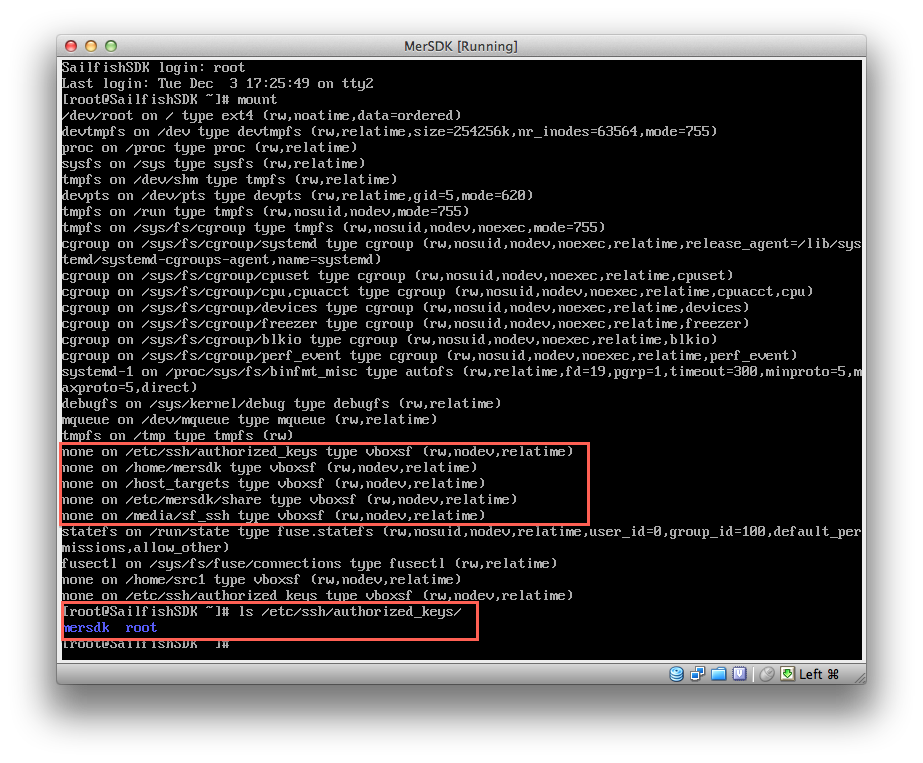
\includegraphics[scale=0.5]{../media/gfx/VirtualBox/vboxmersdkcheckdrives.png} 
  \caption{Check for authorized\_keys.}
  \label{fig:vboxmersdkcheckdrives}
\end{figure}
%
If the drive exists\footnote{It seems that the output of mount does not show it right, even if it is mounted and accessible.}, you can check if the file is accessible.
\begin{lstlisting}[language=bash]
ls -lah /etc/ssh/authorized_keys/mersdk/authorized_keys
ls -lah /etc/ssh/authorized_keys/root/authorized_keys
\end{lstlisting}
%
Handle the other shared folders according to this.
%
Your VM acts strange and you don't know why? Check if updates for VirtualBox are available. If yes, download and install the latest version and don't forget the extension pack.
%
\begin{figure}[H]
  \centering
  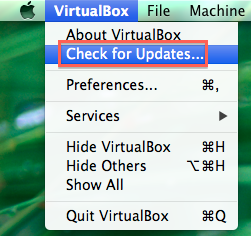
\includegraphics[scale=0.6]{../media/gfx/VirtualBox/vboxisupdateavailable.png} 
  \caption{Check if VirtualBox update is available.}
  \label{fig:vboxisupdateavailable}
\end{figure}
%
\begin{figure}[H]
  \centering
  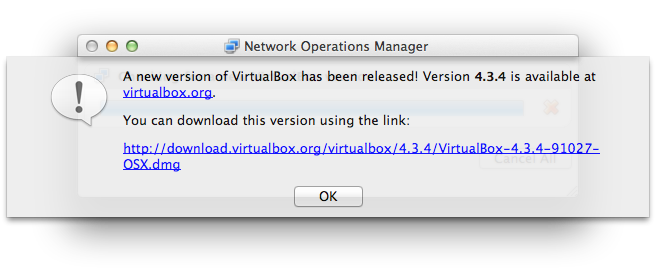
\includegraphics[scale=0.6]{../media/gfx/VirtualBox/vboxupateavailable.png} 
  \caption{Update for VirtualBox is available.}
  \label{fig:vboxupateavailable}
\end{figure}
%
%
\subsubsection{Slow}\label{subsubsec:ts:slowmersdk}
%
I had the situation where everything seems perfect and still it didn't work. For me the last resort was re-installing the VM with the Mer SDK, see section \nameref{sec:uninstall} on page \pageref{sec:uninstall} but even that did not help in the end.
%
One one machine the VM was running but slow\footnote{As in tar pit.}, so every connection attempt timed out. Even control from VirtualBox itself was almost impossible.
%
\begin{figure}[H]
  \centering
  
\includegraphics[scale=0.6]{../media/gfx/VirtualBox/vboxtarpit.png} 
  \caption{VM can not be controlled.}
  \label{fig:vboxtarpit}
\end{figure}
%
This could even happen to a working and running VM to which I successfully logged in via ssh. Working inside the terminal: no problem: compiling: no go.
Until now I found no solution for this.
%
\begin{figure}[H]
  \centering
  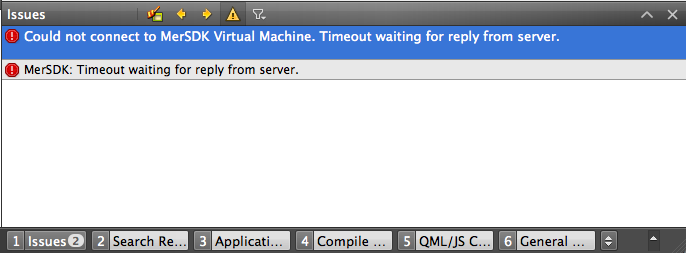
\includegraphics[scale=0.6]{../media/gfx/VirtualBox/MerSDKTimeout.png} 
  \caption{Project ERROR: Could not connect to MerSDK Virtual Machine. Timeout waiting for reply from server.}
  \label{fig:MerSDKTimeout}
\end{figure}
%
This happened on a notebook where the hard drive is clearly a bottleneck but it should nevertheless be fast enough to handle this task\footnote{No SSD, spinning disks with 5400 RPM.}.

If nothing else works, power off the VM from inside VirtualBox. Even that may freeze. When the VM is in state \emph{aborted}, kill VirtualBox and start it again. Now start the VM manually from inside VirtualBox. QtCreator will not recognize such a VM as running. Hit the $\vcenter{\hbox{
\includegraphics[scale=0.6]{../media/gfx/QtCreator/SDKstart.png}}}$ button and after its green again, your good to go.
\\
\\
Funny enough after looking into the logfile\footnote{Have look in the ~/SailfishOS/mersdk/MerSDK/Logs folder} of the VM, I found this message:
%
\begin{lstlisting}[language=tex]
AIOMgr: Host limits number of active IO requests to 16. Expect a performance impact.
\end{lstlisting}
%
After some google'ing I found a hint mentioning the \emph{I/O Host Cache} setting being off\footnote{This was for Vagrant which also utilizes VitualBox.}. So I checked to box for a test.
%
\begin{figure}[H]
  \centering
  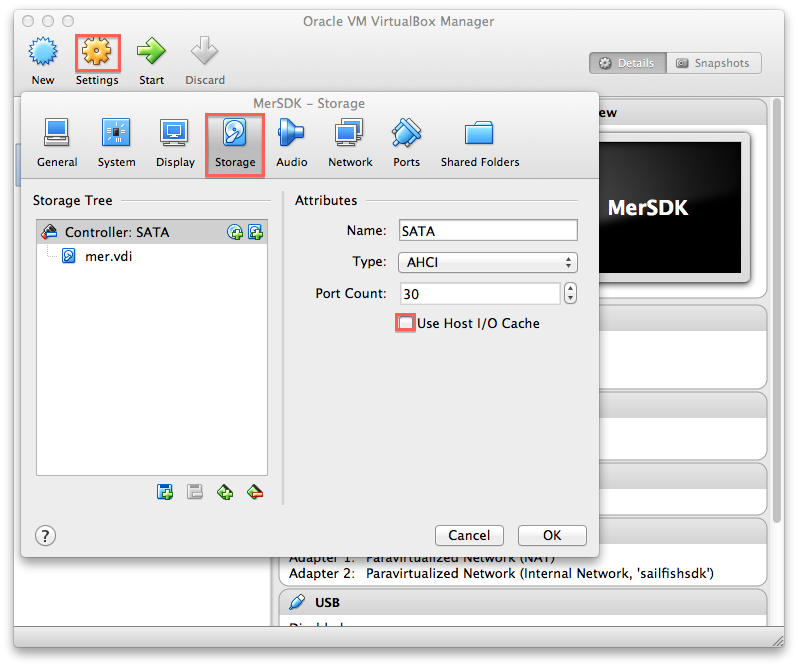
\includegraphics[scale=0.6]{../media/gfx/VirtualBox/IOCache.png} 
  \caption{Turn on the host I/O cache.}
  \label{fig:IOCache}
\end{figure}
%

Inside the VirtualBox manual is a section that may describe the cause for these problems\cite{vbox02}, as it talks about slow disk systems and that is truly the case here\footnote{From the slow notebook hard drive perspective}, but I must admit that I did not experience the mentioned IDE/SATA errors.

I am testing this right now, don't know yet if that really helps = call this experimental.

Open your terminal and run the following commands
%
\begin{lstlisting}[language=bash]
VBoxManage showvminfo "MerSDK"|grep SATA
Storage Controller Name (0):            SATA
SATA (1, 0): /Users/sven/SailfishOS/mersdk/mer.vdi (UUID: fd25a075-e327-46b6-8657-3ab4c4294f94)
# the 1 in 'SATA (1, 0)' is what we are looking for
# it translates to the 1 in 'LUN#1' in the following command
#                                |
#                                +--------------------------------+
#                                                                 |
VBoxManage setextradata "MerSDK" "VBoxInternal/Devices/ahci/0/LUN#1/Config/FlushInterval" 5000000
# reasonable values for FlushInterval are between 1000000 (write often) and 10000000 (write bigger chunks)
# so I chose the middle ground (meanwhile I am at 1000000)
# if it fails after all and your VM refuses to start, you can remove the value with
VBoxManage setextradata "MerSDK" "VBoxInternal/Devices/ahci/0/LUN#1/Config/FlushInterval"
VBoxManage setextradata "MerSDK" "VBoxInternal/Devices/ahci/0/LUN#1/Config/IgnoreFlush"
\end{lstlisting}
%
This didn't solve all my problems so far but the VM got more responsive\footnote{This comes at a price of course, the more often the VM writes the more often it will stress the host machine = your development computer.}.

So far all tweaks have the same effect: they work after I implemented them bot only for a certain time. Then everything goes back to normal =  poor performance or not working at all. But all the problems occur on 1 of 3 OSC machines I've tested the SDK on.

So this could be a some OSX machines problem only.

Another variation of this problem: MerSDK VM starts, I can login via SSH and everything is fine. After starting to build, the SSH session freezes. No CPU spikes, working directly inside the VM is still possible.
%
%
\subsection{Emulator}
%
%
\subsubsection{Deploying offline}
%
When you deploy an app to the emulator\footnote{Deploy happens when you hit \emph{run}.} and the deployment process discovers that you have dependent packages, it tries to download them automatically. That works not so well if you're offline. The following lines could show up in the \emph{Compile Output} tab.
%
\begin{lstlisting}[language=tex]
Status: 	Downloading packages
Package:	qt5-qttest-5.1.0+git17-1.13.1.i486
Results:
Fatal error: Download (curl) error for 'http://releases.sailfishos.org/sdk/latest/jolla/i486/qt/i486/qt5-qttest-5.1.0+git17-1.13.1.i486.rpm':
Error code: Connection failed
Error message: Couldn't resolve host 'releases.sailfishos.org'
\end{lstlisting}
%
At least for the first compilation of your app you may need a connection to the internet.
%
%
\subsubsection{Timeout, emulator offline}
%
The emulator is running as you can see but QtCreator complains that it is not reachable. That is a well known bug, just hit the start button in QtCreator and try again.
%
\subsubsection{Battery life on real device}
%
Some community members have figured out that the NFC chip causes quite heavy battery draining\cite{rj01}. If you don't need the chip for now, there is a way to stop the underlying service. Login your device and enter
%
\begin{lstlisting}[language=bash]
systemctl stop tohd.service
# to stop the service and
systenctl mask tohd.service
# to make the change permanent, so it survives reboots
\end{lstlisting}